% ============================================================================
% TinyRecursiveControl - Architecture Figures
% ============================================================================
% This file contains TikZ diagrams for the TRC paper
% Compile with: pdflatex paper_figures.tex
% ============================================================================

\documentclass[tikz,border=10pt]{standalone}
\usepackage{tikz}
\usepackage{amsmath}
\usepackage{amssymb}
\usetikzlibrary{shapes.geometric, arrows.meta, positioning, calc, fit, backgrounds, decorations.pathreplacing, shadows, patterns}

% Define colors (professional color scheme)
\definecolor{inputcolor}{RGB}{66, 133, 244}      % Google Blue
\definecolor{encodercolor}{RGB}{52, 168, 83}     % Google Green
\definecolor{reasoningcolor}{RGB}{251, 188, 4}   % Google Yellow
\definecolor{decodercolor}{RGB}{234, 67, 53}     % Google Red
\definecolor{outputcolor}{RGB}{156, 39, 176}     % Purple
\definecolor{feedbackcolor}{RGB}{255, 87, 34}    % Deep Orange
\definecolor{latentcolor}{RGB}{0, 150, 136}      % Teal
\definecolor{lightgray}{RGB}{245, 245, 245}
\definecolor{darkgray}{RGB}{97, 97, 97}

\begin{document}

% ============================================================================
% FIGURE 1: Main Architecture Overview (Similar to TRM figure style)
% ============================================================================
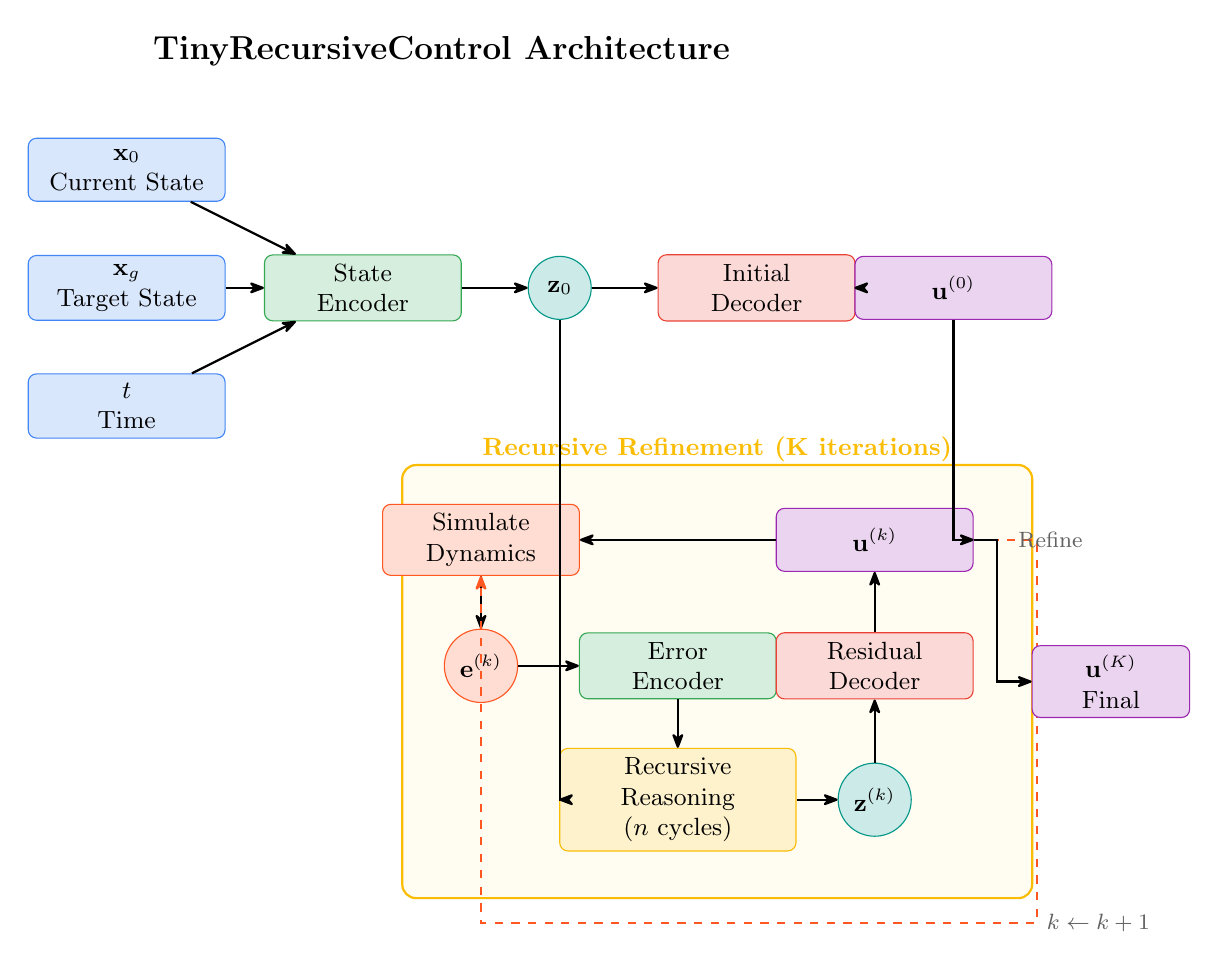
\begin{tikzpicture}[
    node distance=1.5cm,
    >={Stealth[round]},
    box/.style={rectangle, rounded corners=3pt, draw, minimum width=2.5cm, minimum height=0.8cm, align=center, font=\small},
    input/.style={box, fill=inputcolor!20, draw=inputcolor},
    encoder/.style={box, fill=encodercolor!20, draw=encodercolor},
    reasoning/.style={box, fill=reasoningcolor!20, draw=reasoningcolor},
    decoder/.style={box, fill=decodercolor!20, draw=decodercolor},
    output/.style={box, fill=outputcolor!20, draw=outputcolor},
    latent/.style={circle, draw=latentcolor, fill=latentcolor!20, minimum size=0.8cm, font=\small},
    arrow/.style={->, thick},
    dasharrow/.style={->, thick, dashed},
    label/.style={font=\footnotesize, text=darkgray}
]

% Title
\node[font=\large\bfseries] at (4, 5) {TinyRecursiveControl Architecture};

% Inputs
\node[input] (x0) at (0, 3.5) {$\mathbf{x}_0$\\Current State};
\node[input] (xg) at (0, 2) {$\mathbf{x}_g$\\Target State};
\node[input] (t) at (0, 0.5) {$t$\\Time};

% State Encoder
\node[encoder] (enc) at (3, 2) {State\\Encoder};

% Initial Latent
\node[latent] (z0) at (5.5, 2) {$\mathbf{z}_0$};

% Initial Control Generator
\node[decoder] (init) at (8, 2) {Initial\\Decoder};

% Initial Controls
\node[output] (u0) at (10.5, 2) {$\mathbf{u}^{(0)}$};

% Recursive Refinement Box
\begin{scope}[on background layer]
\node[draw=reasoningcolor, thick, rounded corners=5pt, fill=reasoningcolor!5,
      minimum width=8cm, minimum height=5.5cm] (refine_box) at (7.5, -3) {};
\end{scope}
\node[font=\small\bfseries, text=reasoningcolor] at (7.5, -0.05) {Recursive Refinement (K iterations)};

% Inside refinement box
% Dynamics Simulation
\node[box, fill=feedbackcolor!20, draw=feedbackcolor] (sim) at (4.5, -1.2) {Simulate\\Dynamics};

% Error
\node[latent, fill=feedbackcolor!20, draw=feedbackcolor] (e) at (4.5, -2.8) {$\mathbf{e}^{(k)}$};

% Error Encoder
\node[encoder] (err_enc) at (7, -2.8) {Error\\Encoder};

% Reasoning Module
\node[reasoning, minimum width=3cm, minimum height=1.2cm] (reason) at (7, -4.5) {Recursive\\Reasoning\\($n$ cycles)};

% Updated Latent
\node[latent] (zk) at (9.5, -4.5) {$\mathbf{z}^{(k)}$};

% Residual Decoder
\node[decoder] (res_dec) at (9.5, -2.8) {Residual\\Decoder};

% Control Update
\node[output] (uk) at (9.5, -1.2) {$\mathbf{u}^{(k)}$};

% Arrows - Initial path
\draw[arrow] (x0) -- (enc);
\draw[arrow] (xg) -- (enc);
\draw[arrow] (t) -- (enc);
\draw[arrow] (enc) -- (z0);
\draw[arrow] (z0) -- (init);
\draw[arrow] (init) -- (u0);

% Arrow to refinement
\draw[arrow] (u0) -- (10.5, -1.2) -- (uk);

% Refinement loop arrows
\draw[arrow] (uk) -- (sim);
\draw[arrow] (sim) -- (e);
\draw[arrow] (e) -- (err_enc);
\draw[arrow] (err_enc) -- (reason);
\draw[arrow] (z0) -- (5.5, -4.5) -- (reason);
\draw[arrow] (reason) -- (zk);
\draw[arrow] (zk) -- (res_dec);
\draw[arrow] (res_dec) -- (uk);

% Loop back arrow
\draw[dasharrow, feedbackcolor] (uk.east) -- ++(0.8, 0) |- ($(refine_box.south east) + (-0.5, -0.3)$)
    node[pos=0.5, right, label] {$k \leftarrow k+1$}
    -| ($(sim.south) + (0, -0.5)$) -- (sim.south);

% Final output
\node[output, minimum width=2cm] (final) at (12.5, -3) {$\mathbf{u}^{(K)}$\\Final};
\draw[arrow, thick] (uk.east) -- ++(0.3, 0) |- (final);

% Labels
\node[label, anchor=west] at (11.2, -1.2) {Refine};

\end{tikzpicture}

\newpage

% ============================================================================
% FIGURE 2: Recursive Refinement Process (Detailed Flow)
% ============================================================================
\begin{tikzpicture}[
    node distance=1.2cm,
    >={Stealth[round]},
    iteration/.style={rectangle, rounded corners=5pt, draw=darkgray, minimum width=3cm, minimum height=2.5cm, align=center},
    step/.style={rectangle, rounded corners=2pt, draw, minimum width=2.2cm, minimum height=0.5cm, align=center, font=\scriptsize},
    arrow/.style={->, thick},
    label/.style={font=\footnotesize}
]

% Title
\node[font=\large\bfseries] at (6, 4) {Recursive Refinement Process};

% Iteration boxes
\foreach \i in {0, 1, 2} {
    \pgfmathtruncatemacro{\x}{\i * 4}

    % Box
    \node[iteration, fill=lightgray] (iter\i) at (\x, 0) {};

    % Label
    \ifnum\i=0
        \node[font=\small\bfseries] at (\x, 1.5) {Initial};
    \else
        \node[font=\small\bfseries] at (\x, 1.5) {Iteration $k=\i$};
    \fi
}

% Dots for more iterations
\node[font=\large] at (10, 0) {$\cdots$};

% Final iteration
\node[iteration, fill=outputcolor!10] (iterK) at (12, 0) {};
\node[font=\small\bfseries] at (12, 1.5) {Iteration $k=K$};

% Steps in each iteration
% Initial
\node[step, fill=encodercolor!20] at (0, 0.5) {Encode State};
\node[step, fill=decodercolor!20] at (0, -0.3) {Generate $\mathbf{u}^{(0)}$};
\node[step, fill=white] at (0, -1.1) {---};

% Iteration 1
\node[step, fill=feedbackcolor!20] at (4, 0.5) {Simulate};
\node[step, fill=reasoningcolor!20] at (4, -0.3) {Reason ($n\times$)};
\node[step, fill=decodercolor!20] at (4, -1.1) {Refine $\mathbf{u}^{(1)}$};

% Iteration 2
\node[step, fill=feedbackcolor!20] at (8, 0.5) {Simulate};
\node[step, fill=reasoningcolor!20] at (8, -0.3) {Reason ($n\times$)};
\node[step, fill=decodercolor!20] at (8, -1.1) {Refine $\mathbf{u}^{(2)}$};

% Iteration K
\node[step, fill=feedbackcolor!20] at (12, 0.5) {Simulate};
\node[step, fill=reasoningcolor!20] at (12, -0.3) {Reason ($n\times$)};
\node[step, fill=outputcolor!30] at (12, -1.1) {Final $\mathbf{u}^{(K)}$};

% Arrows between iterations
\draw[arrow] (iter0) -- (iter1);
\draw[arrow] (iter1) -- (iter2);
\draw[arrow] (9.5, 0) -- (10.5, 0);
\draw[arrow, thick, outputcolor] (iterK) -- ++(1.5, 0) node[right, label] {Output};

% Error decrease visualization
\node[font=\small\bfseries] at (6, -2.5) {Trajectory Error};
\draw[->] (-0.5, -3) -- (13.5, -3) node[right, label] {Iteration};
\draw[->] (-0.5, -3) -- (-0.5, -4.5) node[above, label] {Error};

% Error bars (decreasing)
\fill[decodercolor!70] (0, -3) rectangle (0.5, -4.3);
\fill[decodercolor!70] (4, -3) rectangle (4.5, -3.8);
\fill[decodercolor!70] (8, -3) rectangle (8.5, -3.4);
\fill[outputcolor!70] (12, -3) rectangle (12.5, -3.15);

\node[label] at (0.25, -4.5) {$e_0$};
\node[label] at (4.25, -4.0) {$e_1$};
\node[label] at (8.25, -3.6) {$e_2$};
\node[label] at (12.25, -3.35) {$e_K$};

% Caption
\node[font=\footnotesize, text width=12cm, align=center] at (6, -5.3) {
    Each iteration: (1) Simulate trajectory with current controls,
    (2) Recursive reasoning updates latent $\mathbf{z}$ with error feedback,
    (3) Residual decoder refines controls. Error decreases monotonically.
};

\end{tikzpicture}

\newpage

% ============================================================================
% FIGURE 3: Comparison - TRM vs TRC
% ============================================================================
\begin{tikzpicture}[
    node distance=1cm,
    >={Stealth[round]},
    box/.style={rectangle, rounded corners=3pt, draw, minimum width=2cm, minimum height=0.6cm, align=center, font=\scriptsize},
    arrow/.style={->, thick},
    label/.style={font=\footnotesize}
]

% Title
\node[font=\large\bfseries] at (5.5, 5.5) {TRM (Discrete) vs TRC (Control)};

% Left side - TRM
\node[font=\bfseries] at (2, 4.5) {TRM (Original)};
\begin{scope}[on background layer]
\node[draw=darkgray, rounded corners=5pt, fill=inputcolor!5,
      minimum width=4.5cm, minimum height=6cm] at (2, 1) {};
\end{scope}

% TRM components
\node[box, fill=inputcolor!20] (trm_x) at (2, 3.5) {Question $\mathbf{x}$};
\node[box, fill=latentcolor!20] (trm_z) at (2, 2.3) {Latent $\mathbf{z}$};
\node[box, fill=reasoningcolor!20] (trm_r) at (2, 1.1) {Reasoning};
\node[box, fill=outputcolor!20] (trm_y) at (2, -0.1) {Answer $\mathbf{y}$};
\node[box, fill=white, draw=darkgray, dashed] (trm_out) at (2, -1.3) {Discrete Output};

\draw[arrow] (trm_x) -- (trm_z);
\draw[arrow] (trm_z) -- (trm_r);
\draw[arrow] (trm_r) -- (trm_y);
\draw[arrow] (trm_y) -- (trm_out);
\draw[dasharrow, reasoningcolor] (trm_y.west) -- ++(-0.5, 0) |- (trm_r.west);

% Right side - TRC
\node[font=\bfseries] at (9, 4.5) {TRC (Ours)};
\begin{scope}[on background layer]
\node[draw=encodercolor, rounded corners=5pt, fill=encodercolor!5,
      minimum width=4.5cm, minimum height=6cm] at (9, 1) {};
\end{scope}

% TRC components
\node[box, fill=inputcolor!20] (trc_x) at (9, 3.5) {$\mathbf{x}_0, \mathbf{x}_g, t$};
\node[box, fill=latentcolor!20] (trc_z) at (9, 2.3) {Latent $\mathbf{z}$};
\node[box, fill=reasoningcolor!20] (trc_r) at (9, 1.1) {Reasoning};
\node[box, fill=decodercolor!20] (trc_u) at (9, -0.1) {Controls $\mathbf{u}$};
\node[box, fill=feedbackcolor!20] (trc_sim) at (11.5, 1.1) {Dynamics\\$f(\cdot)$};
\node[box, fill=feedbackcolor!20] (trc_e) at (11.5, 2.3) {Error $\mathbf{e}$};
\node[box, fill=outputcolor!30, draw=outputcolor] (trc_out) at (9, -1.3) {Continuous Output};

\draw[arrow] (trc_x) -- (trc_z);
\draw[arrow] (trc_z) -- (trc_r);
\draw[arrow] (trc_r) -- (trc_u);
\draw[arrow] (trc_u) -- (trc_out);

% Feedback loop (NOVEL)
\draw[arrow, feedbackcolor, thick] (trc_u.east) -- ++(0.3, 0) |- (trc_sim.south);
\draw[arrow, feedbackcolor, thick] (trc_sim) -- (trc_e);
\draw[arrow, feedbackcolor, thick] (trc_e.west) -- ($(trc_r.east) + (0, 0.3)$);

% Novel contribution highlight
\draw[decorate, decoration={brace, amplitude=5pt, mirror}, feedbackcolor, thick]
    (10.7, 0.5) -- (10.7, 2.8) node[midway, right=5pt, font=\scriptsize, text=feedbackcolor] {Novel};

% Legend
\node[font=\small\bfseries] at (5.5, -2.5) {Key Differences};
\node[font=\scriptsize, text width=8cm, align=left] at (5.5, -3.5) {
    \textbullet\ TRM: Discrete outputs (Sudoku cells, puzzle answers)\\
    \textbullet\ TRC: Continuous outputs (control sequences $\mathbf{u} \in \mathbb{R}^{T \times d_u}$)\\
    \textbullet\ \textcolor{feedbackcolor}{\textbf{TRC Novel:}} Trajectory feedback guides refinement
};

\end{tikzpicture}

\newpage

% ============================================================================
% FIGURE 4: Method Comparison Diagram
% ============================================================================
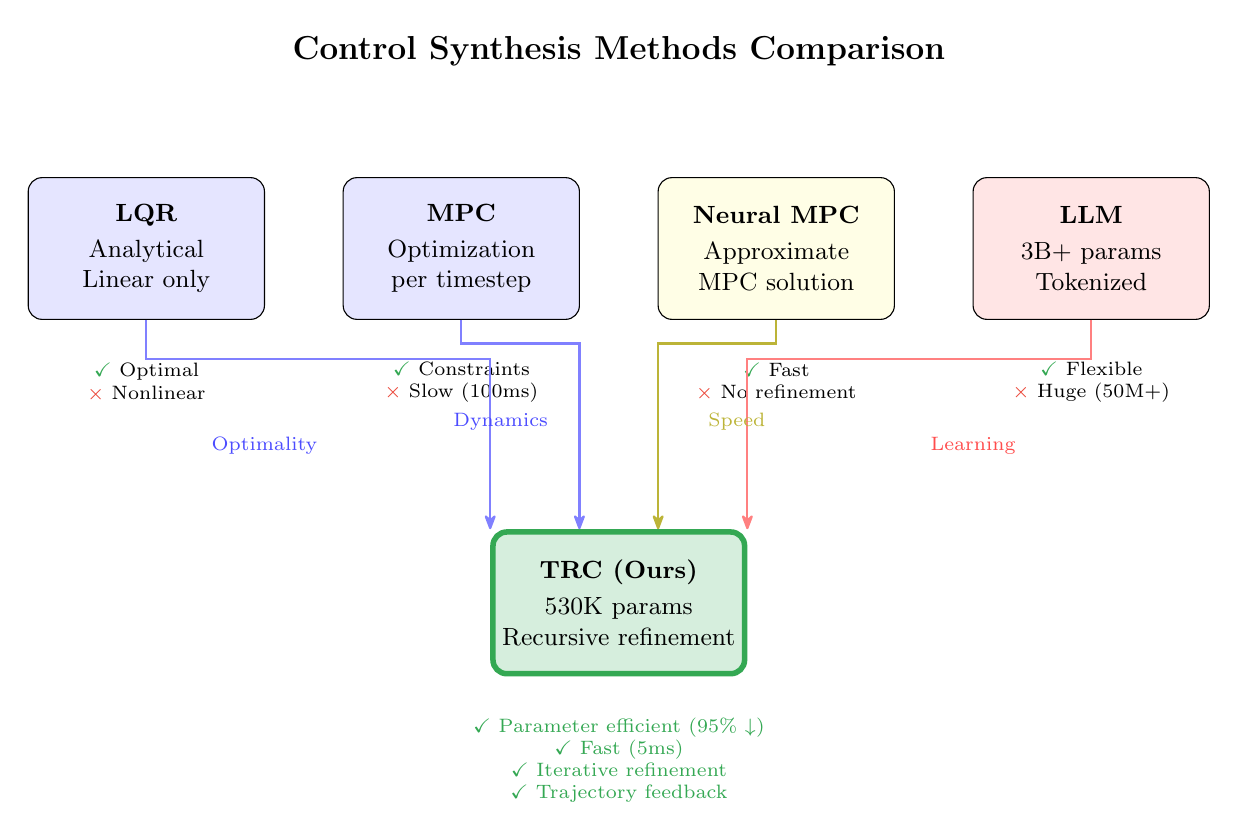
\begin{tikzpicture}[
    node distance=1.5cm,
    >={Stealth[round]},
    method/.style={rectangle, rounded corners=5pt, draw, minimum width=3cm, minimum height=1.8cm, align=center, font=\small},
    arrow/.style={->, thick},
    label/.style={font=\scriptsize}
]

% Title
\node[font=\large\bfseries] at (6, 5) {Control Synthesis Methods Comparison};

% LQR
\node[method, fill=blue!10] (lqr) at (0, 2.5) {
    \textbf{LQR}\\[2pt]
    Analytical\\
    Linear only
};
\node[label, text width=2.5cm, align=center] at (0, 0.8) {
    \textcolor{encodercolor}{\checkmark} Optimal\\
    \textcolor{decodercolor}{$\times$} Nonlinear
};

% MPC
\node[method, fill=blue!10] (mpc) at (4, 2.5) {
    \textbf{MPC}\\[2pt]
    Optimization\\
    per timestep
};
\node[label, text width=2.5cm, align=center] at (4, 0.8) {
    \textcolor{encodercolor}{\checkmark} Constraints\\
    \textcolor{decodercolor}{$\times$} Slow (100ms)
};

% Neural MPC
\node[method, fill=yellow!10] (nmpc) at (8, 2.5) {
    \textbf{Neural MPC}\\[2pt]
    Approximate\\
    MPC solution
};
\node[label, text width=2.5cm, align=center] at (8, 0.8) {
    \textcolor{encodercolor}{\checkmark} Fast\\
    \textcolor{decodercolor}{$\times$} No refinement
};

% LLM
\node[method, fill=red!10] (llm) at (12, 2.5) {
    \textbf{LLM}\\[2pt]
    3B+ params\\
    Tokenized
};
\node[label, text width=2.5cm, align=center] at (12, 0.8) {
    \textcolor{encodercolor}{\checkmark} Flexible\\
    \textcolor{decodercolor}{$\times$} Huge (50M+)
};

% TRC (highlighted)
\node[method, fill=encodercolor!20, draw=encodercolor, line width=2pt] (trc) at (6, -2) {
    \textbf{TRC (Ours)}\\[2pt]
    530K params\\
    Recursive refinement
};
\node[label, text width=4cm, align=center, text=encodercolor] at (6, -4) {
    \textcolor{encodercolor}{\checkmark} Parameter efficient (95\% $\downarrow$)\\
    \textcolor{encodercolor}{\checkmark} Fast (5ms)\\
    \textcolor{encodercolor}{\checkmark} Iterative refinement\\
    \textcolor{encodercolor}{\checkmark} Trajectory feedback
};

% Arrows showing TRC combines benefits
\draw[arrow, blue!50] (lqr.south) -- ++(0, -0.5) -| (trc.north west);
\draw[arrow, blue!50] (mpc.south) -- ++(0, -0.3) -| ($(trc.north) + (-0.5, 0)$);
\draw[arrow, yellow!70!black] (nmpc.south) -- ++(0, -0.3) -| ($(trc.north) + (0.5, 0)$);
\draw[arrow, red!50] (llm.south) -- ++(0, -0.5) -| (trc.north east);

% Labels on arrows
\node[label, blue!70] at (1.5, 0) {Optimality};
\node[label, blue!70] at (4.5, 0.3) {Dynamics};
\node[label, yellow!70!black] at (7.5, 0.3) {Speed};
\node[label, red!70] at (10.5, 0) {Learning};

\end{tikzpicture}

\newpage

% ============================================================================
% FIGURE 5: Inner Reasoning Block Detail
% ============================================================================
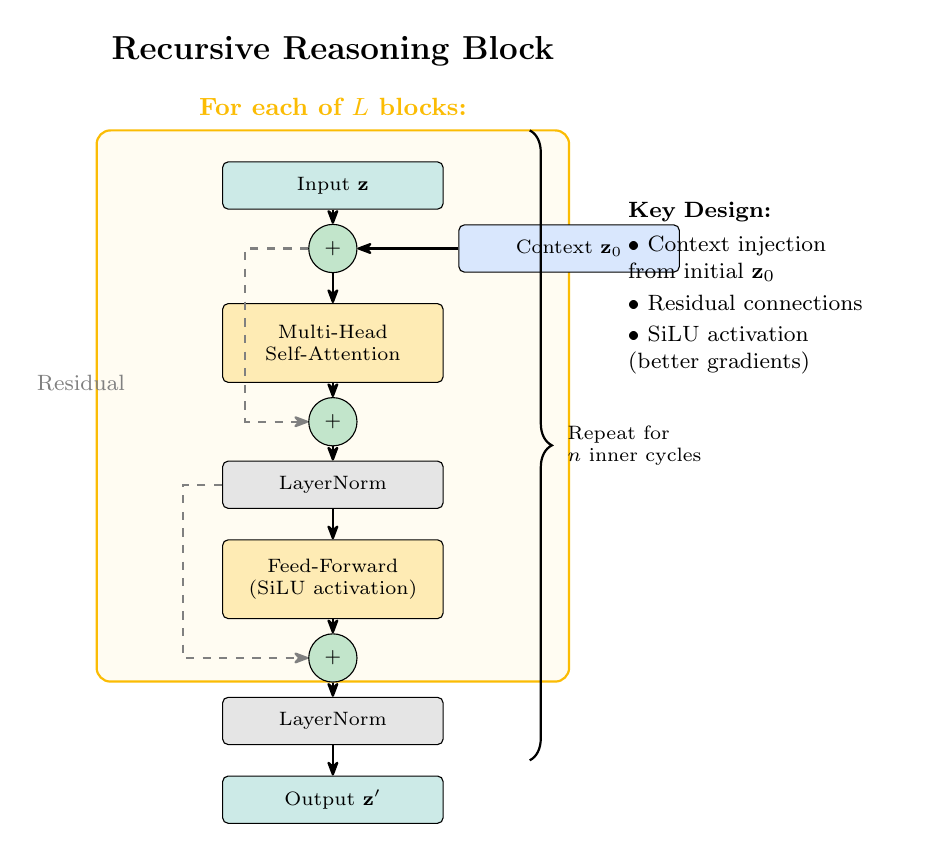
\begin{tikzpicture}[
    node distance=0.8cm,
    >={Stealth[round]},
    block/.style={rectangle, rounded corners=2pt, draw, minimum width=2.8cm, minimum height=0.6cm, align=center, font=\scriptsize},
    op/.style={circle, draw, minimum size=0.4cm, font=\scriptsize},
    arrow/.style={->, thick},
    label/.style={font=\footnotesize}
]

% Title
\node[font=\large\bfseries] at (4, 5.5) {Recursive Reasoning Block};

% Main block outline
\begin{scope}[on background layer]
\node[draw=reasoningcolor, thick, rounded corners=5pt, fill=reasoningcolor!5,
      minimum width=6cm, minimum height=7cm] at (4, 1) {};
\end{scope}
\node[font=\small\bfseries, text=reasoningcolor] at (4, 4.8) {For each of $L$ blocks:};

% Input
\node[block, fill=latentcolor!20] (input) at (4, 3.8) {Input $\mathbf{z}$};

% Context injection
\node[op, fill=encodercolor!30] (add1) at (4, 3) {$+$};
\node[block, fill=inputcolor!20] (ctx) at (7, 3) {Context $\mathbf{z}_0$};

% Multi-head attention
\node[block, fill=reasoningcolor!30, minimum height=1cm] (attn) at (4, 1.8) {Multi-Head\\Self-Attention};

% Add & Norm 1
\node[op, fill=encodercolor!30] (add2) at (4, 0.8) {$+$};
\node[block, fill=gray!20] (norm1) at (4, 0) {LayerNorm};

% FFN
\node[block, fill=reasoningcolor!30, minimum height=1cm] (ffn) at (4, -1.2) {Feed-Forward\\(SiLU activation)};

% Add & Norm 2
\node[op, fill=encodercolor!30] (add3) at (4, -2.2) {$+$};
\node[block, fill=gray!20] (norm2) at (4, -3) {LayerNorm};

% Output
\node[block, fill=latentcolor!20] (output) at (4, -4) {Output $\mathbf{z}'$};

% Arrows
\draw[arrow] (input) -- (add1);
\draw[arrow] (ctx) -- (add1);
\draw[arrow] (add1) -- (attn);
\draw[arrow] (attn) -- (add2);
\draw[arrow] (add2) -- (norm1);
\draw[arrow] (norm1) -- (ffn);
\draw[arrow] (ffn) -- (add3);
\draw[arrow] (add3) -- (norm2);
\draw[arrow] (norm2) -- (output);

% Residual connections
\draw[arrow, gray, dashed] (add1.west) -- ++(-0.8, 0) |- (add2.west);
\draw[arrow, gray, dashed] (norm1.west) -- ++(-0.5, 0) |- (add3.west);

% Labels for residual
\node[label, gray] at (0.8, 1.3) {Residual};

% Annotations
\node[label, text width=3.5cm, align=left] at (9.5, 2.5) {
    \textbf{Key Design:}\\[3pt]
    \textbullet\ Context injection\\
    from initial $\mathbf{z}_0$\\[2pt]
    \textbullet\ Residual connections\\[2pt]
    \textbullet\ SiLU activation\\
    (better gradients)
};

% Loop indicator
\draw[decorate, decoration={brace, amplitude=8pt}, thick]
    (6.5, 4.5) -- (6.5, -3.5) node[midway, right=10pt, font=\scriptsize, text width=2cm, align=left] {
        Repeat for\\$n$ inner cycles
    };

\end{tikzpicture}

\newpage

% ============================================================================
% FIGURE 6: Weight Sharing Visualization
% ============================================================================
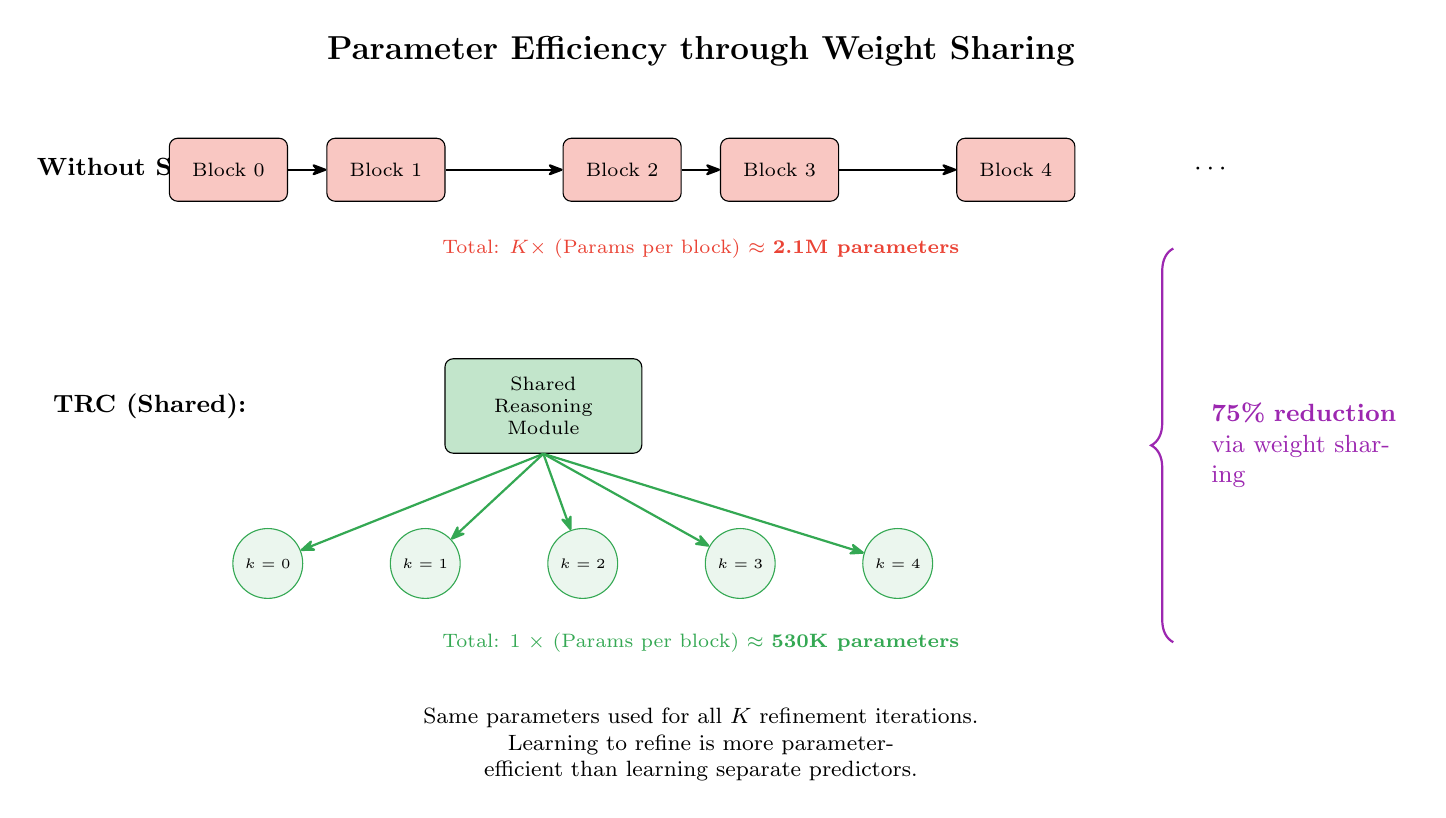
\begin{tikzpicture}[
    node distance=1cm,
    >={Stealth[round]},
    block/.style={rectangle, rounded corners=3pt, draw, minimum width=1.5cm, minimum height=0.8cm, align=center, font=\scriptsize},
    arrow/.style={->, thick},
    label/.style={font=\scriptsize}
]

% Title
\node[font=\large\bfseries] at (6, 4) {Parameter Efficiency through Weight Sharing};

% Without weight sharing (top)
\node[font=\small\bfseries] at (-1, 2.5) {Without Sharing:};

\foreach \i in {0, 1, 2, 3, 4} {
    \pgfmathtruncatemacro{\x}{\i * 2.5}
    \node[block, fill=decodercolor!30] (block\i) at (\x, 2.5) {Block $\i$};
}
\node at (12.5, 2.5) {$\cdots$};

% Arrows
\draw[arrow] (block0) -- (block1);
\draw[arrow] (block1) -- (block2);
\draw[arrow] (block2) -- (block3);
\draw[arrow] (block3) -- (block4);

% Parameter count
\node[label, text=decodercolor] at (6, 1.5) {Total: $K \times$ (Params per block) $\approx$ \textbf{2.1M parameters}};

% With weight sharing (bottom)
\node[font=\small\bfseries] at (-1, -0.5) {TRC (Shared):};

% Single block
\node[block, fill=encodercolor!30, minimum width=2.5cm, minimum height=1.2cm] (shared) at (4, -0.5) {
    Shared\\Reasoning\\Module
};

% Multiple uses
\foreach \i in {0, 1, 2, 3, 4} {
    \pgfmathtruncatemacro{\x}{\i * 2}
    \node[circle, draw=encodercolor, fill=encodercolor!10, minimum size=0.6cm, font=\tiny] (use\i) at (\x + 0.5, -2.5) {$k=\i$};
}

% Arrows from shared to uses
\foreach \i in {0, 1, 2, 3, 4} {
    \draw[arrow, encodercolor] (shared.south) -- (use\i);
}

% Parameter count
\node[label, text=encodercolor] at (6, -3.5) {Total: 1 $\times$ (Params per block) $\approx$ \textbf{530K parameters}};

% Savings highlight
\draw[decorate, decoration={brace, amplitude=8pt, mirror}, thick, outputcolor]
    (12, 1.5) -- (12, -3.5) node[midway, right=10pt, font=\small, text=outputcolor, text width=2.5cm, align=left] {
        \textbf{75\% reduction}\\
        via weight sharing
    };

% Note
\node[font=\footnotesize, text width=10cm, align=center] at (6, -4.8) {
    Same parameters used for all $K$ refinement iterations.\\
    Learning to refine is more parameter-efficient than learning separate predictors.
};

\end{tikzpicture}

\newpage

% ============================================================================
% FIGURE 7: Trajectory Feedback Mechanism (Novel Contribution)
% ============================================================================
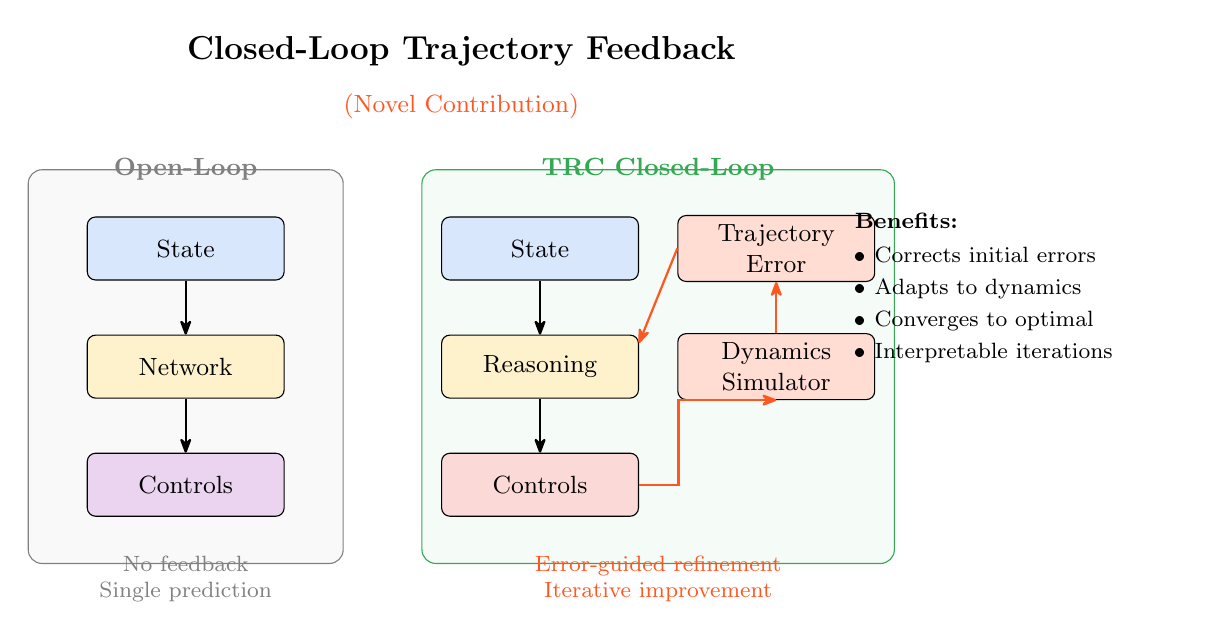
\begin{tikzpicture}[
    node distance=1cm,
    >={Stealth[round]},
    box/.style={rectangle, rounded corners=3pt, draw, minimum width=2.5cm, minimum height=0.8cm, align=center, font=\small},
    arrow/.style={->, thick},
    label/.style={font=\footnotesize}
]

% Title
\node[font=\large\bfseries] at (5, 5.5) {Closed-Loop Trajectory Feedback};
\node[font=\small, text=feedbackcolor] at (5, 4.8) {(Novel Contribution)};

% Left: Open-loop (previous methods)
\begin{scope}[on background layer]
\node[draw=gray, rounded corners=5pt, fill=gray!5,
      minimum width=4cm, minimum height=5cm] at (1.5, 1.5) {};
\end{scope}
\node[font=\small\bfseries, gray] at (1.5, 4) {Open-Loop};

\node[box, fill=inputcolor!20] (ol_in) at (1.5, 3) {State};
\node[box, fill=reasoningcolor!20] (ol_net) at (1.5, 1.5) {Network};
\node[box, fill=outputcolor!20] (ol_out) at (1.5, 0) {Controls};

\draw[arrow] (ol_in) -- (ol_net);
\draw[arrow] (ol_net) -- (ol_out);

\node[label, gray, text width=3cm, align=center] at (1.5, -1.2) {
    No feedback\\
    Single prediction
};

% Right: Closed-loop (TRC)
\begin{scope}[on background layer]
\node[draw=encodercolor, rounded corners=5pt, fill=encodercolor!5,
      minimum width=6cm, minimum height=5cm] at (7.5, 1.5) {};
\end{scope}
\node[font=\small\bfseries, text=encodercolor] at (7.5, 4) {TRC Closed-Loop};

\node[box, fill=inputcolor!20] (cl_in) at (6, 3) {State};
\node[box, fill=reasoningcolor!20] (cl_net) at (6, 1.5) {Reasoning};
\node[box, fill=decodercolor!20] (cl_ctrl) at (6, 0) {Controls};
\node[box, fill=feedbackcolor!20] (cl_sim) at (9, 1.5) {Dynamics\\Simulator};
\node[box, fill=feedbackcolor!20] (cl_err) at (9, 3) {Trajectory\\Error};

\draw[arrow] (cl_in) -- (cl_net);
\draw[arrow] (cl_net) -- (cl_ctrl);
\draw[arrow, feedbackcolor, thick] (cl_ctrl.east) -- ++(0.5, 0) |- (cl_sim.south);
\draw[arrow, feedbackcolor, thick] (cl_sim) -- (cl_err);
\draw[arrow, feedbackcolor, thick] (cl_err.west) -- ($(cl_net.east) + (0, 0.3)$);

\node[label, text=feedbackcolor, text width=3.5cm, align=center] at (7.5, -1.2) {
    Error-guided refinement\\
    Iterative improvement
};

% Benefit annotations
\node[font=\footnotesize, text width=4cm, align=left] at (12, 2.5) {
    \textbf{Benefits:}\\[3pt]
    \textbullet\ Corrects initial errors\\[2pt]
    \textbullet\ Adapts to dynamics\\[2pt]
    \textbullet\ Converges to optimal\\[2pt]
    \textbullet\ Interpretable iterations
};

\end{tikzpicture}

\newpage

% ============================================================================
% FIGURE 8: Complete System Flow (Publication-Ready)
% ============================================================================
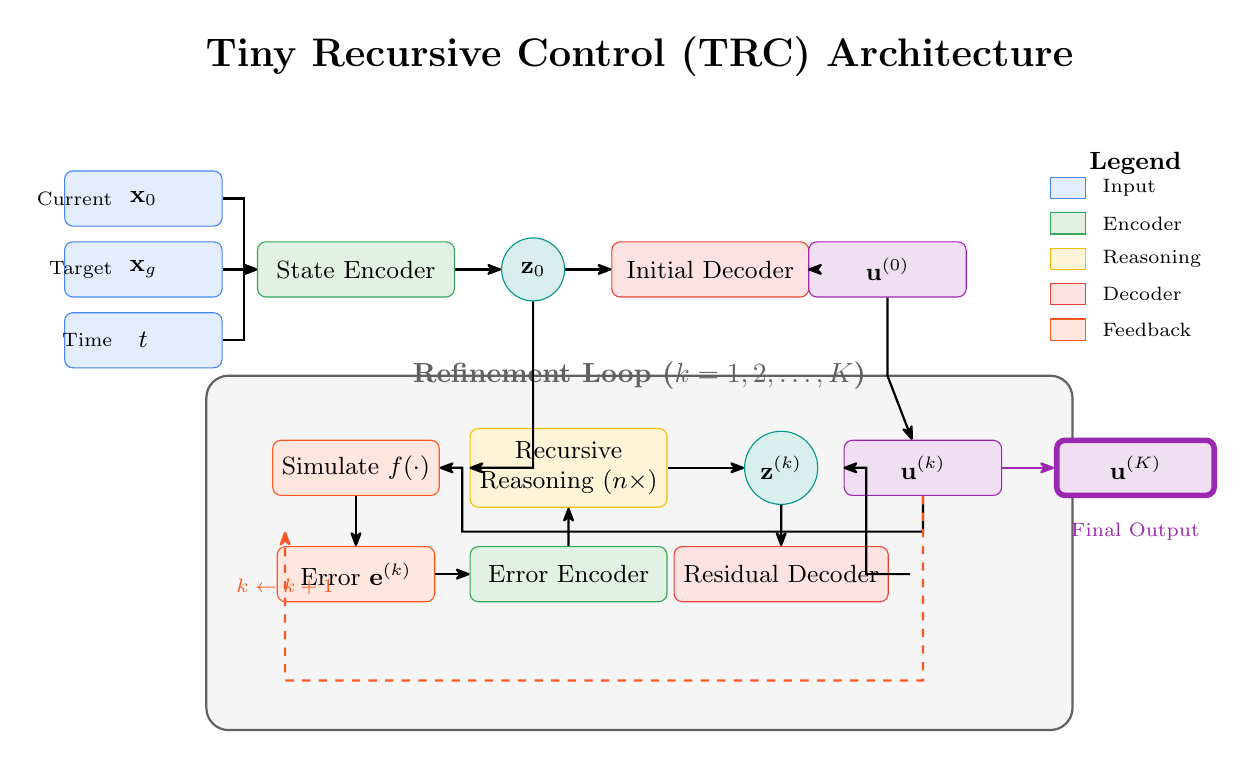
\begin{tikzpicture}[
    scale=0.9,
    node distance=1cm,
    >={Stealth[round]},
    input/.style={rectangle, rounded corners=3pt, draw=inputcolor, fill=inputcolor!15, minimum width=2cm, minimum height=0.7cm, align=center, font=\small},
    encoder/.style={rectangle, rounded corners=3pt, draw=encodercolor, fill=encodercolor!15, minimum width=2.5cm, minimum height=0.7cm, align=center, font=\small},
    reasoning/.style={rectangle, rounded corners=3pt, draw=reasoningcolor, fill=reasoningcolor!15, minimum width=2.5cm, minimum height=0.7cm, align=center, font=\small},
    decoder/.style={rectangle, rounded corners=3pt, draw=decodercolor, fill=decodercolor!15, minimum width=2.5cm, minimum height=0.7cm, align=center, font=\small},
    output/.style={rectangle, rounded corners=3pt, draw=outputcolor, fill=outputcolor!15, minimum width=2cm, minimum height=0.7cm, align=center, font=\small},
    feedback/.style={rectangle, rounded corners=3pt, draw=feedbackcolor, fill=feedbackcolor!15, minimum width=2cm, minimum height=0.7cm, align=center, font=\small},
    latent/.style={circle, draw=latentcolor, fill=latentcolor!15, minimum size=0.8cm, font=\small},
    arrow/.style={->, thick},
    label/.style={font=\scriptsize}
]

% Title
\node[font=\Large\bfseries] at (7, 7) {Tiny Recursive Control (TRC) Architecture};

% === Input Section ===
\node[input] (x0) at (0, 5) {$\mathbf{x}_0$};
\node[input] (xg) at (0, 4) {$\mathbf{x}_g$};
\node[input] (t) at (0, 3) {$t$};

\node[label, anchor=east] at (-0.3, 5) {Current};
\node[label, anchor=east] at (-0.3, 4) {Target};
\node[label, anchor=east] at (-0.3, 3) {Time};

% === State Encoder ===
\node[encoder] (state_enc) at (3, 4) {State Encoder};

% === Initial Latent ===
\node[latent] (z0) at (5.5, 4) {$\mathbf{z}_0$};

% === Initial Decoder ===
\node[decoder] (init_dec) at (8, 4) {Initial Decoder};

% === Initial Controls ===
\node[output] (u0) at (10.5, 4) {$\mathbf{u}^{(0)}$};

% === Refinement Loop (Main Box) ===
\begin{scope}[on background layer]
\node[draw=darkgray, thick, rounded corners=8pt, fill=lightgray,
      minimum width=11cm, minimum height=4.5cm] at (7, 0) {};
\end{scope}
\node[font=\bfseries, darkgray] at (7, 2.5) {Refinement Loop ($k = 1, 2, \ldots, K$)};

% Inside refinement loop
\node[feedback] (sim) at (3, 1.2) {Simulate $f(\cdot)$};
\node[feedback] (err) at (3, -0.3) {Error $\mathbf{e}^{(k)}$};
\node[encoder] (err_enc) at (6, -0.3) {Error Encoder};
\node[reasoning, minimum height=1cm] (reason) at (6, 1.2) {Recursive\\Reasoning ($n\times$)};
\node[latent] (zk) at (9, 1.2) {$\mathbf{z}^{(k)}$};
\node[decoder] (res_dec) at (9, -0.3) {Residual Decoder};
\node[output] (uk) at (11, 1.2) {$\mathbf{u}^{(k)}$};

% Arrows - Main flow
\draw[arrow] (x0.east) -- ++(0.3, 0) |- (state_enc);
\draw[arrow] (xg) -- (state_enc);
\draw[arrow] (t.east) -- ++(0.3, 0) |- (state_enc);
\draw[arrow] (state_enc) -- (z0);
\draw[arrow] (z0) -- (init_dec);
\draw[arrow] (init_dec) -- (u0);

% Arrow into refinement
\draw[arrow] (u0) -- (10.5, 2.5) -- (uk);

% Refinement internal arrows
\draw[arrow] (uk.south) -- (11, 0.3) -- (4.5, 0.3) -- (4.5, 1.2) -- (sim);
\draw[arrow] (sim) -- (err);
\draw[arrow] (err) -- (err_enc);
\draw[arrow] (err_enc) -- (reason);
\draw[arrow] (z0) -- (5.5, 1.2) -- (reason);
\draw[arrow] (reason) -- (zk);
\draw[arrow] (zk) -- (9, 0.4) -- (res_dec);
\draw[arrow] (res_dec.east) -- ++(0.3, 0) -- (10.2, -0.3) -- (10.2, 1.2) -- (uk);

% Loop continuation arrow
\draw[arrow, feedbackcolor, thick, dashed] (uk.south) -- (11, -1.8) -- (2, -1.8)
    -- (2, 0.3) node[pos=0.75, below, label] {$k \leftarrow k+1$};

% Final output
\node[output, draw=outputcolor, line width=2pt] (final) at (14, 1.2) {$\mathbf{u}^{(K)}$};
\draw[arrow, outputcolor, thick] (uk) -- (final);

\node[label, text=outputcolor] at (14, 0.3) {Final Output};

% Legend
\node[font=\small\bfseries] at (14, 5.5) {Legend};
\draw[fill=inputcolor!15, draw=inputcolor] (12.8, 5) rectangle (13.3, 5.3);
\node[label, anchor=west] at (13.4, 5.15) {Input};
\draw[fill=encodercolor!15, draw=encodercolor] (12.8, 4.5) rectangle (13.3, 4.8);
\node[label, anchor=west] at (13.4, 4.65) {Encoder};
\draw[fill=reasoningcolor!15, draw=reasoningcolor] (12.8, 4) rectangle (13.3, 4.3);
\node[label, anchor=west] at (13.4, 4.15) {Reasoning};
\draw[fill=decodercolor!15, draw=decodercolor] (12.8, 3.5) rectangle (13.3, 3.8);
\node[label, anchor=west] at (13.4, 3.65) {Decoder};
\draw[fill=feedbackcolor!15, draw=feedbackcolor] (12.8, 3) rectangle (13.3, 3.3);
\node[label, anchor=west] at (13.4, 3.15) {Feedback};

\end{tikzpicture}

\end{document}
